\chapter{Introduction}

\section{Background}
Stethoscopes reveal vital diagnostic information about a patient’s heart, lungs and airways.  At the Royal Melbourne Hospital, patients with infectious and potentially fatal diseases, like Ebola, are going to treat in isolation rooms which keep at negative pressure so that diseases don’t get out and it will be preventing from outbreak. 
In the isolation rooms, doctors require a stethoscope to use. However, the conventional stethoscope is unable to be used because doctors need to wear full body protection suits equipped with fans to keep the suit at positive pressure to keep the diseases out of the suits.  There are some commercial available electronic stethoscopes require Bluetooth ear pieces or a cable to a computer.  Nevertheless, those available electronic stethoscopes are not feasible in the isolation room since there is the risk of contaminating when doctors take off head piece and doctors want to avoid earphones as they need to avoid touching their face. Moreover, the price of the commercial available electronic stethoscopes are too expensive which is approximately 800 dollars each.  Thus, there is no suitable stethoscopes can be used in the isolation room.

\section{Project Aims}
This project aims to modify a new cheaper stethoscope that uses electronic sensors to detect and transmit sound data to a speaker interface. This electronic stethoscope will be designed for use in isolation rooms at Royal Melbourne Hospital, enabling doctors to perform auscultations without compromising the integrity of their isolation suits. 

\subsection{Product Requirements}
The stethoscope must not compromise the isolation suites used in the isolation room. The design should have a diaphragm that operate like a traditional stethoscope so that the doctors are familiar with the product and it does not change the behaviour of doctor using traditional stethoscope. The sound signal should be adjustable and output via a wired speaker and wireless speaker.  Besides, the electronic stethoscope can be powered by a battery or external wall adapter. And the battery must last life time of a single patient. The size of the product should be small enough so that it can be held by a single hand. At last, the cost of the product should be cheaper than the current available electronic stethoscope.

\subsection{Product Specification}
\subsubsection{Sound Signal collection}
Sound Signal is collected by using a conventional diaphragm (Fig.~\ref{fig:conventional_stethoscope}). A traditional stethoscope can be easier to modify to a wireless stethoscope by attach the diaphragm to the product.
\begin{figure}[!htbp]
	\centering
		\fbox{
		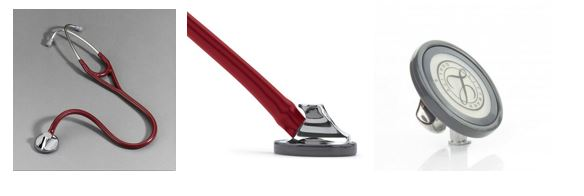
\includegraphics[width=140mm]{conventional_stethoscope.jpg}
		}
	\caption{Conventional stethoscope}
	\label{fig:conventional_stethoscope}
\end{figure}

\subsubsection{Signal processing}
Microcontroller is included in the design in order to do digital signal processing. Removing noise, cancelling feedback and other signal processing may be required when the product operates in different environments. Digital Signal Processing is more flexible than in physical signal processing

\subsubsection{Size}
The electronic board is approximately 15cm length and 5 cm wide and covered by a plastic cylinder. A cone or a short part of tube is provided to connect the diaphragm and the plastic cylinder 
 
\subsubsection{Power supply}
Two different power supply options are provided.
A battery or rechargeable battery makes it more portable.
External wall plug-in adapter makes it last long time operation.

\subsubsection{Output format}
Sound signal form diaphragm can be played through a wired speaker and a Bluetooth speaker.
Volume can be adjustable.

\subsubsection{Indication}
There are different LEDs to indicate different operation stages, such as power on, Bluetooth operation and so on.

\subsubsection{Cost}
The total cost of product to modify the conventional stethoscope is lower than the half price of the current available wireless stethoscope since the stethoscope may be modified to use for training purpose.

\begin{figure}[!htbp]
	\centering
		\fbox{
		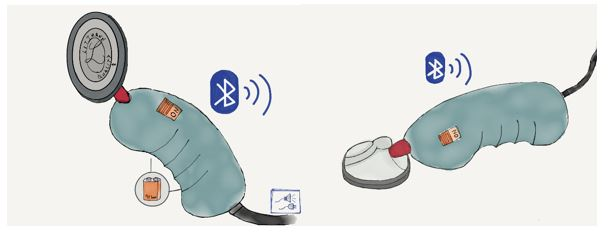
\includegraphics[width=140mm]{design_idea.jpg}
		}
	\caption{Idea to modify conventional sethoscope for wireless sound transmission}
	\label{fig:design_idea}
\end{figure}